% Options for packages loaded elsewhere
\PassOptionsToPackage{unicode}{hyperref}
\PassOptionsToPackage{hyphens}{url}
\PassOptionsToPackage{dvipsnames,svgnames*,x11names*}{xcolor}
%
\documentclass[
  11pt,
]{article}

\usepackage{lmodern}
\usepackage{amssymb,amsmath}
\usepackage{ifxetex,ifluatex}
\ifnum 0\ifxetex 1\fi\ifluatex 1\fi=0 % if pdftex
  \usepackage[T1]{fontenc}
  \usepackage[utf8]{inputenc}
  \usepackage{textcomp} % provide euro and other symbols
\else % if luatex or xetex
  \usepackage{unicode-math}
  \defaultfontfeatures{Scale=MatchLowercase}
  \defaultfontfeatures[\rmfamily]{Ligatures=TeX,Scale=1}
  \setmainfont[]{cochineal}
  \setsansfont[]{Fira Sans}
\fi

% Use upquote if available, for straight quotes in verbatim environments
\IfFileExists{upquote.sty}{\usepackage{upquote}}{}
\IfFileExists{microtype.sty}{% use microtype if available
  \usepackage[]{microtype}
  \UseMicrotypeSet[protrusion]{basicmath} % disable protrusion for tt fonts
}{}
\makeatletter
\@ifundefined{KOMAClassName}{% if non-KOMA class
  \IfFileExists{parskip.sty}{%
    \usepackage{parskip}
  }{% else
    \setlength{\parindent}{0pt}
    \setlength{\parskip}{6pt plus 2pt minus 1pt}}
}{% if KOMA class
  \KOMAoptions{parskip=half}}
\makeatother
\usepackage{xcolor}
\IfFileExists{xurl.sty}{\usepackage{xurl}}{} % add URL line breaks if available
\IfFileExists{bookmark.sty}{\usepackage{bookmark}}{\usepackage{hyperref}}
\hypersetup{
  pdftitle={Résumé},
  pdfauthor={Caleb Williams},
  colorlinks=true,
  linkcolor=Maroon,
  filecolor=Maroon,
  citecolor=Blue,
  urlcolor=blue,
  pdfcreator={LaTeX via pandoc}}
\urlstyle{same} % disable monospaced font for URLs
\usepackage[margin=1in]{geometry}
\setlength{\emergencystretch}{3em} % prevent overfull lines
\providecommand{\tightlist}{%
  \setlength{\itemsep}{0pt}\setlength{\parskip}{0pt}}
\setcounter{secnumdepth}{-\maxdimen} % remove section numbering

\title{Résumé}
\usepackage{authblk}
                        \author{Caleb Williams}
            \date{12/2/2020 -- Update before applying}


%% should be top-aligned in case of uneven vertical length)
\newenvironment{columns}[1][]{}{}
%%
\newenvironment{column}[1]{\begin{minipage}[t]{#1}\ignorespaces}{%
\end{minipage}
\ifhmode\unskip\fi
\aftergroup\useignorespacesandallpars}
%%
\def\useignorespacesandallpars#1\ignorespaces\fi{%
#1\fi\ignorespacesandallpars}
%%
\makeatletter
\def\ignorespacesandallpars{%
  \@ifnextchar\par
    {\expandafter\ignorespacesandallpars\@gobble}%
    {}%
}
\makeatother

% Use fontawesome. Note: you'll need TeXLive 2015. Update.
\usepackage{fontawesome}

% Mess with sections
\usepackage{titlesec}
\usepackage{sectsty}
% \sectionfont{\rmfamily\mdseries\large\bf\underline}
\sectionfont{\normalfont\sffamily\large\bfseries\sectionrule{0pt}{0pt}{-4pt}{1pt}}
\subsectionfont{\rmfamily\mdseries\normalsize\scshape}
\titlespacing\section{0pt}{12pt plus 4pt minus 2pt}{4pt plus 2pt minus 2pt}
\titlespacing\subsection{0pt}{12pt plus 4pt minus 2pt}{4pt plus 2pt minus 2pt}

\usepackage{enumitem}
\setlist[itemize]{leftmargin=*}

\usepackage{graphicx}
\usepackage{tikz}
\usepackage{tikzpagenodes}
\usetikzlibrary{calc} 


% Make AP style (kinda) dates for the updated/today field

\usepackage{datetime}
\newdateformat{apstylekinda}{%
  \shortmonthname[\THEMONTH]. \THEDAY, \THEYEAR}

% Fancyhdr, as I tend to do with these personal documents.
\usepackage{fancyhdr,lastpage}
\pagestyle{fancy}
\renewcommand{\headrulewidth}{0.0pt}
\renewcommand{\footrulewidth}{0.0pt}
\lhead{}
\chead{}
\rhead{}
\lfoot{
\cfoot{\scriptsize  Caleb Williams - Résumé - \emph{Updated:} \apstylekinda\today }}
\rfoot{\scriptsize \thepage/{\hypersetup{linkcolor=black}\pageref{LastPage}}}



% Always load hyperref last.
\usepackage{hyperref}
\PassOptionsToPackage{usenames,dvipsnames}{color} % color is loaded by hyperref

\hypersetup{unicode=true,
            pdftitle={Caleb Williams  (R\'{e}sum\'{e})},
            pdfauthor={Caleb Williams},
            colorlinks=true,
            linkcolor=Maroon,
            citecolor=Blue,
            urlcolor=blue,
            breaklinks=true, bookmarks=true}

\begin{document}
% shift=(current page.north east)
%\begin{wrapfigure}{r}{\textwidth}

\begin{tikzpicture}[remember picture,overlay, shift={(7in,-0.25in)}]
    \clip (0,0) circle (1.75cm) node {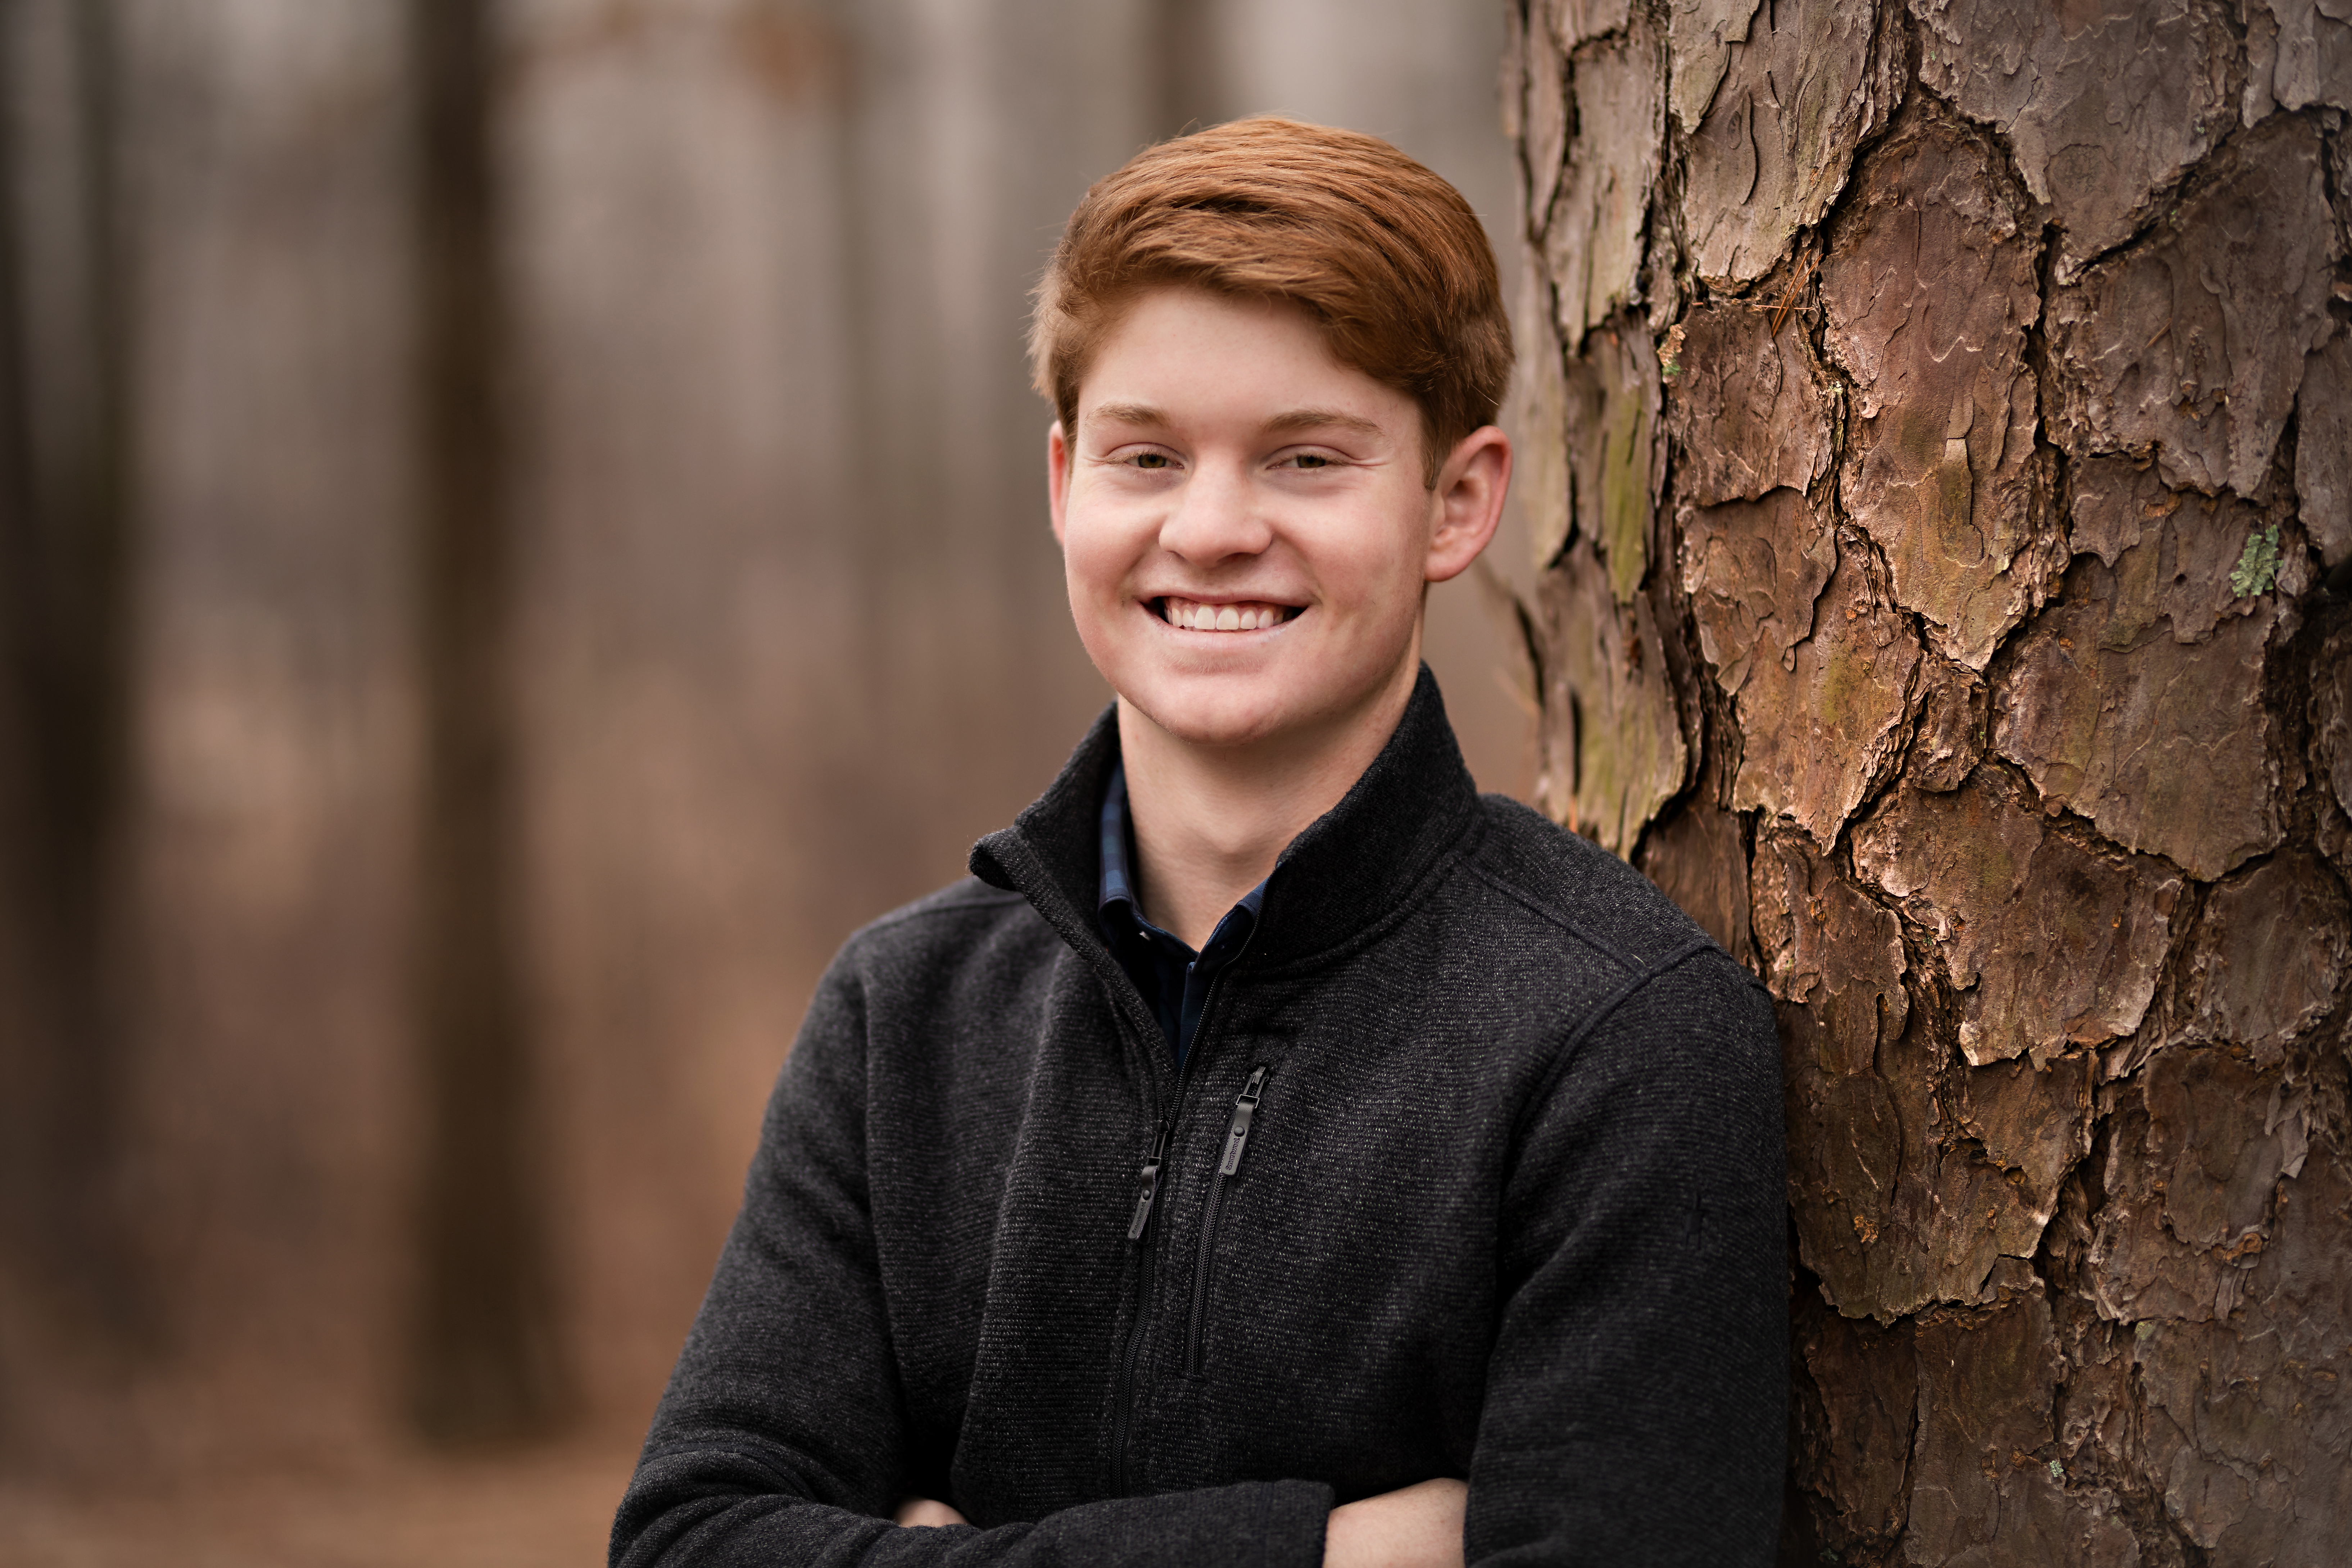
\includegraphics[width=.2\textwidth]{CalebWilliams-Pic.jpg}};
\end{tikzpicture}

 % includephoto
%\end{wrapfigure}

\flushleft{\huge \bfseries Caleb Williams}

\flushleft{\footnotesize

\faEnvelopeO \hspace{1 mm} \href{mailto:}{\tt \href{mailto:jcw068@uark.edu}{\nolinkurl{jcw068@uark.edu}}} \hspace{1 mm}
\faPhone \hspace{1 mm} 870-530-8229 \hspace{1 mm}
\faMapMarker \hspace{1 mm} 110 N Stadium, Fayetteville, AR \hspace{1 mm}
}
\vspace{-1em}
\flushleft{\footnotesize
 
\faTwitter \hspace{1 mm} \href{http://twitter.com/}{\tt } \hspace{1 mm}
\faLinkedin \hspace{1 mm} \href{https://www.linkedin.com/in/john-williams-4398961ba}{\tt john-williams-4398961ba} \hspace{1 mm}
\faGithub \hspace{1 mm} \href{http://github.com/Calebwilliams67}{\tt Calebwilliams67} \hspace{1 mm}
}

\begin{column}{0.60\textwidth}

\hypertarget{professional-experience}{%
\section{Professional Experience}\label{professional-experience}}

\hypertarget{park-maintenance-2018}{%
\subsection{\texorpdfstring{\textbf{Park Maintenance
(2018)}}{Park Maintenance (2018)}}\label{park-maintenance-2018}}

Jonesboro Department of Parks and Recreation --- Jonesboro, Arkansas

\begin{itemize}
\tightlist
\item
  Maintained 7 pavilions at Craighead Forest Park~\\
  through landscaping, cleaning, and operating machines.
\item
  Worked in teams on multiple strenuous project.
\item
  Self-paced work environment where reliability~\\
  and work ethic were key.
\end{itemize}

\hypertarget{real-estate-office-assistant-2019-2020}{%
\subsection{\texorpdfstring{\textbf{Real Estate Office Assistant
(2019-2020)}}{Real Estate Office Assistant (2019-2020)}}\label{real-estate-office-assistant-2019-2020}}

Jonesboro Select Real Estate --- Jonesboro, Arkansas

\begin{itemize}
\tightlist
\item
  Received office phone calls\\
  recording information and relaying it.
\item
  Created flyers and powerpoints\\
  for open houses, closings, and listings
\item
  Captured photos of listings to be published
\end{itemize}

\end{column}

\begin{column}{0.02\textwidth}

~

\end{column}

\begin{column}{0.38\textwidth}

\hypertarget{education}{%
\section{Education}\label{education}}

\hypertarget{highschool}{%
\subsection{\texorpdfstring{\textbf{Highschool}}{Highschool}}\label{highschool}}

Academies at Jonesboro High School --- Jonesboro\\
GPA: 4.17/4.00 ACT: 32\\
Graduated: May 2020

\hypertarget{b.s.-in-data-science}{%
\subsection{\texorpdfstring{\textbf{B.S. in Data
Science}}{B.S. in Data Science}}\label{b.s.-in-data-science}}

University of Arkansas --- Fayetteville \emph{Honors Program}\\
GPA : Will be updated

\hypertarget{technical-skills}{%
\section{Technical Skills}\label{technical-skills}}

\begin{itemize}
\tightlist
\item
  Programming: Python, R, TeX,~\\
  PowerShell, Bash, RStudio, Visual Studio Code and Microsoft Excel.
\item
  Data: importation, manipulation, transformation, visualization, and
  communication.
\item
  Managing Project Environments
\item
  Advanced Quantitative Analysis
\item
  Complex Problem Solving
\end{itemize}

\hypertarget{awards-and-distinctions}{%
\section{Awards and Distinctions}\label{awards-and-distinctions}}

\begin{itemize}
\tightlist
\item
  Chancellor's Community~\\
  Scholarship
\item
  Governor's Distinguished~\\
  Scholarship
\item
  Northeast Arkansas Alumni\\
  Chapter Scholarship
\end{itemize}

\end{column}

\end{document}

